%% LaTeX2e class for student theses
%% sections/content.tex
%% 
%% Karlsruhe Institute of Technology
%% Institute for Program Structures and Data Organization
%% Chair for Software Design and Quality (SDQ)
%%
%% Dr.-Ing. Erik Burger
%% burger@kit.edu
%% burger@kit.edu
%%
%% Version 1.3.3, 2018-04-17


\chapter{Untersuchung von nachrichtenbasierter Middleware}

Auswahl von MOMs

Vorstellung der MOMs

- best practices

- Benchmarks vorstellen

- interessante Ergebnisse der jeweiligen MQ zeigen die spaeter versucht werden sollen zu modellieren

Vergleich der MOMs

\label{ch:momsysteme}
\section{Anforderungen an MOMs}
Da es eine Vielzahl von MOMs gibt, muss zunächst eine Auswahl stattfinden. Dazu werden im ersten Schritt der Masterarbeit Anforderungen erarbeitet, die ein MOM erfüllen muss, damit sie in Betracht kommt. Im Rahmen des Proposals wurde sich bereits mit der Frage auseinander gesetzt und die folgenden Anforderungen erarbeitet:
\begin{itemize}
\item Die MOM sollte \textbf{Open Source} sein.
\item Sie sollte eine \textbf{weite Verbreitung} haben. Um dies einzuschätzen zu können sollen verschiedene Entwicklerforen wie Stackoverflow und Stachshare untersucht werden, sowie die Literatur in diesem Bereich.
\item %Da sowohl das Experimentsystem eine Java und das Evaluierungssystem eine C++ Implementierung besitzen sollte 
Die MOM sollte \textbf{Programmiersprachen unabhängig} sein.
\item Sich in \textbf{aktiver Entwicklung} befinden.
\item Bereits gesammelte \textbf{Erfahrung} mit MOMs.
\end{itemize}
%- bestimmte Protokolle unterstuetzen \\ %(https://www.predic8.de/activemq-hornetq-rabbitmq-apollo-qpid-vergleich.htm)

%\section{Auswahl der MOMs}
%In diesem Schritt sollen zwei bis drei MOMs ausgewählt werden. Dabei sollen die zuvor erarbeiteten Anforderungen einbezogen werden. Da sich bereits im Rahmen des Proposals mit dem Thema auseinander gesetzt wurde, wurden bereits drei starke Kandidaten identifiziert, die die bereits erarbeiteten Anforderungen erfüllen.
Im Folgenden sollen zwei Systeme untersucht werden, die diese Anforderungen erfuellen.

\section{RabbitMQ}
RabbitMQ ist, mit 35,000 aktiven Produktivumgebungen, eine der am weitesten verbreitete MOM. 
RabbitMQ ist eine Open-Source-MOM, die seit 2007 entwickelt wird \cite{rabbitmq}. Das Ziel von RabbitMQ ist es allgemein einsetzbar zu sein. Deshalb wird eine Vielzahl an Protokollen unterstützt, unter anderem das AMQP (Advanced Message Queuing Protocol) Protokoll \cite{amqp}. AMQP ist unabhängig von einer Programmiersprache und definiert das Verhalten des Senders und Empfängers, um Interoperabilität zu erreichen, damit MOMs sich untereinander verständigen können. RabbitMQ kann in verteilten Systemen und in unterschiedlichen Konfigurationen eingesetzt werden, um hohe Anforderungen an Skalierbarkeit und Zuverlässigkeit zu erfüllen. In \autoref{img:rmq_architecture} ist die Architectur von RMQ abgebildet. Dabei faellt auf, dass in RabbitMQ Nachrichten nicht direkt an eine Warteschlange gesendet werden, sondern an einen Exchange. Dieser ist für das richtige weiterleiten an die passende Warteschlange verantwortlich. Warteschlangen werden mithilfe von Bindings an ein Exchange gebunden und mithilfe von Routing-Schlüsseln identifiziert. RabbitMQ unterscheidet zwischen vier verschiedenen Exchanges:
\begin{itemize}
    \item Direkt: Hierbei meldet sich eine Warteschlange mit einem bestimmten Routing-Schlüssel (RK) X beim Exchange an. Wenn eine Nachricht mit einem RK Y ankommt, wird sie nur an die Warteschlange gesendet, wenn die RKs X und Y übereinstimmen.
    \item Topic: Die Warteschlange ist mit einem Binding an den Exchange gebunden. Nachrichten werden wieder anhand des RK weitergeleitet. Der RK muss nicht mehr genau passen, sondern muss auf ein bestimmtes Muster aufweisen.
    \item Fanout: Die ankommende Nachricht wird an alle am Exchange angemeldeten Warteschlangen gesendet. Der RK wird dabei ignoriert.
    \item Header:
\end{itemize}
\begin{figure}
\center
  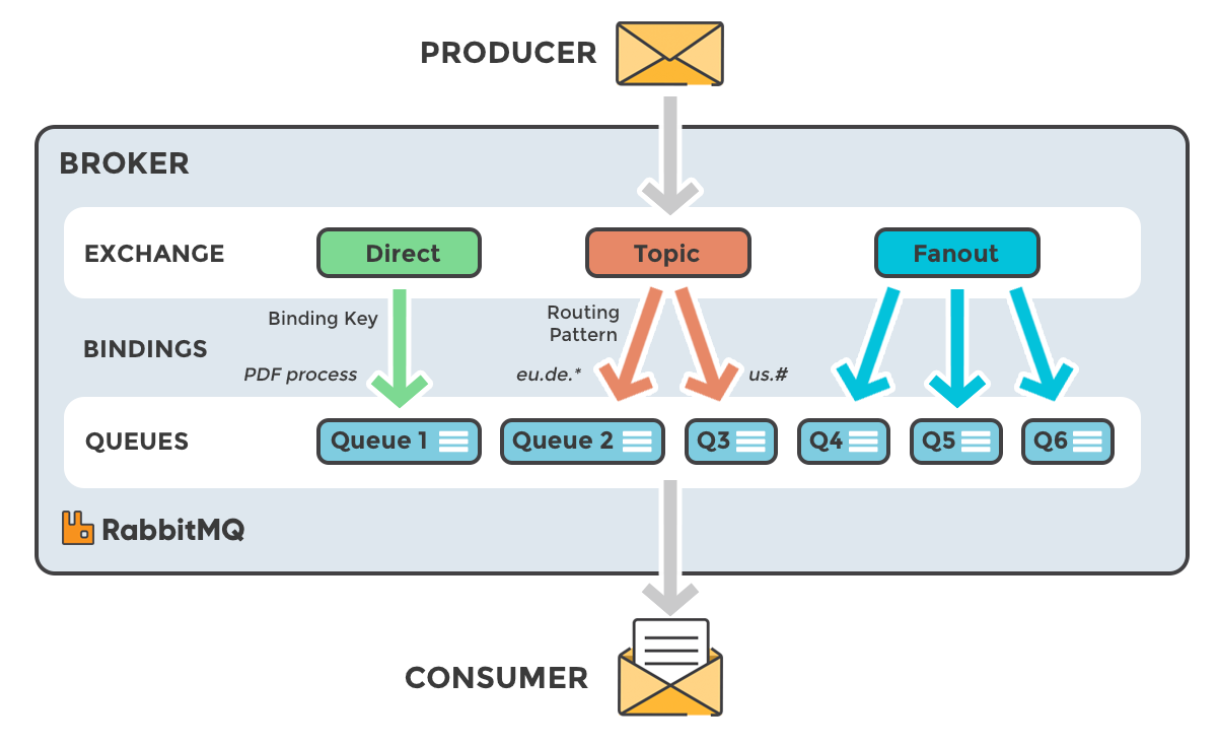
\includegraphics[width=1\textwidth]{images/rmq_architecture.png}
  \caption{Maximaler Durchsatz}
  \label{img:rmq_architecture}
\end{figure}
%https://www.cloudamqp.com/blog/2015-05-18-part1-rabbitmq-for-beginners-what-is-rabbitmq.html
\subsection{Best Practises}
%https://www.cloudamqp.com/blog/2018-01-08-part2-rabbitmq-best-practice-for-high-performance.html
Da in dieser Arbeit der Fokus auf der Performanz verschiedener MOMs liegt, wurden zunÄchst die Möglichkeiten untersucht, mit denen eine hohe Performanz erreicht werden kann. Dazu wurde vorwiegend Literatur von RabbitMQ herangezogen. Die folgenden Einstellungen bzw. EIgenschaften konnten indentifiziert werden.
\begin{itemize}
    \item kurze Warteschlangen
    \item setze Warteschlangen länge
    \item keine lazy queues
    \item mehrere Warteschlangen und Verbraucher
\end{itemize}
Diese Eigenschaften wurden im folgenden untersucht um zu prüfen ob sie einen messbaren einfluss auf die Performanz haben.

\section{Kafka}
Kafka wurde bei LinkedIn entwickelt und hauptsächlich für die Protokollierung eingesetzt \cite{kafka}. Die grundlegenden Merkmale hinter Kafka sind das Performanz über Zuverlässigkeit gestellt wird und dadurch hoher Durchsatz und niedrige Latenzzeiten ermöglicht werden. Kafka kann sowohl für Online- als auch für die Offline-Protokoll-ierung eingesetzt werden. In ihrer Arbeit zeigen die Entwickler, dass Kafka mindestens doppelt so viele Nachrichten senden und vier mal so viele Nachrichten empfangen kann, als ActiveMQ und RabbitMQ. In \autoref{img:kafka_architecture} ist die Kafka Architektur abgebildet. Dabei sendet ein Sender an ein Cluster. Dieses Cluster verteilt die Nachricht an die verschiedenen Empfaenger. 
\begin{figure}
\center
  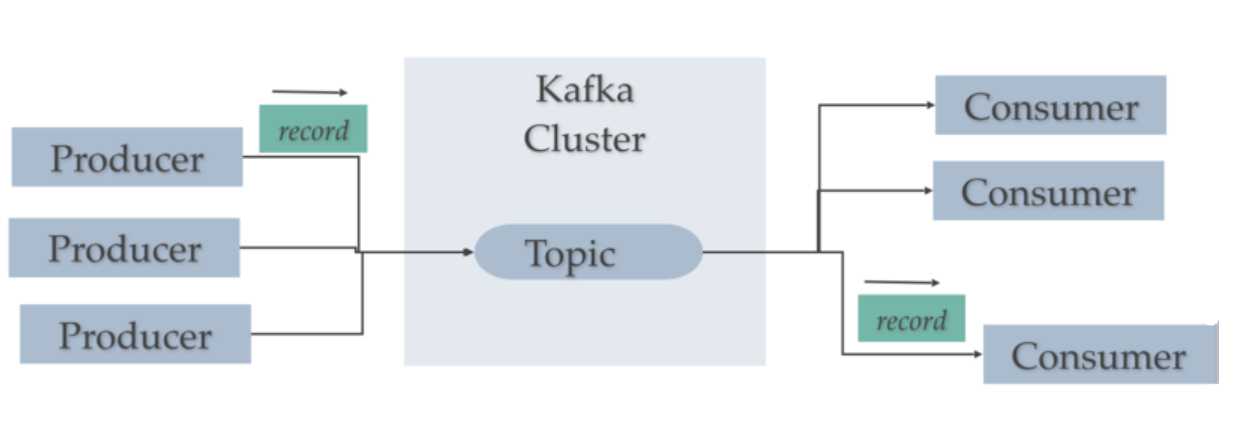
\includegraphics[width=1\textwidth]{images/kafka_architecture.png}
  \caption{Maximaler Durchsatz}
  \label{img:kafka_architecture}
\end{figure}

\subsection{Best Practice}

\section{Benchmark}
Im Folgenden sollen in erster Linie die Standard Konfigurationen betrachtet werden.
\subsection{Testmaschinen}
\label{sec:testmachine}
In diesem Abschnitt sollen die benutzten Maschinen Dokumentiert werden, mit denen die verschiedenen MOMs untersucht wurden:
\begin{itemize}
    \item Testmaschine A: Localhost
    \item Testmaschine B: VM
\end{itemize}

\subsection{RMQ}
Im Folgenden soll besprochen werden, welche Eigenschaften in RMQ Auswirkungen auf die Performanz haben. Dazu wurde das Performanz Test Werkzeug von RMQ benutzt. Dieses erlaubt es die gesendeten und empfangenen Nachrichten und ihre Latenz zu messen. Dabei ist die Zeit gemeint, die eine Nachricht braucht bis sie vom Empfänger aus der Warteschlange herausgenommen wird, nachdem sie vom Sender dort abgelegt wurde. Das Werkzeug kann konfiguriert werden um bestimmte Szenarien zu simulieren. Unter anderem laesst sich die Anzahl zu sendenden und zu empfangenen Nachrichte pro Sekunde einstellen. Eine weitere Konfiguration ist das einstellen bestimmte Nachrichtengroessen. Im Folgenden sollen die Ergebnisse der Messungen vorgestellt werden. Dabei werden die einzelnen Ergebnisse und ihr Versuchsaufbau vorgestellt.
%\subsection{Ergebnisse}
%In diesem Abschnitt werden die Ergebnisse der Performanzmessungen von RMQ vorgestellt. 
Die benutzten Systeme sind in \autoref{sec:testmachine} beschrieben. Sollten sich bestimmte Szenarien auf verschiedenen Maschinen unterschiedlich verhalten, wird dies angemerkt. Falls keine Anmerkung erfolgt, heisst das, dass bei der Messungen kein Einfluss erkannt werden konnte. Jedes Ergebnis wird wie folgt vorgestellt: Zunaechst wird das jeweilige Szeanario vorgestellt. Im naechsten Schritt werden die Beobachtungen beschrieben und im Anschluss das daraus resultierende Ergebnis.



\subsubsection{Latenz einer Nachricht}
Zunaechst soll geprueft werden wie die Latenz einer einzelnen Nachricht ist. Dabei wurde auch die groesse einer Nachricht betrachtet. Dazu wurde die Senderate auf eine Nachricht pro Sekunde reduziert und die Nachrichtengroesse varriert zwischen 100 Byte und 100.000 Bytes.
%B
Die Ergebnisse sind in \autoref{img:senderate1-A} zu sehen. Dabei ist zu sehen, dass die Latenz mit Ansteigen der Groesse auch waechst. 
%Im durchshnitt kann man eine Latenz von 2627 Mikrosekunden beobachten. In \autoref{img:senderate1-B} sind die Ergebnisse mit Testsystem B zu sehen. Hier wird im durchshnitt eine hoehere Latenz von 29237 Mikrosekunden beobachten. 
\begin{figure}
\center
  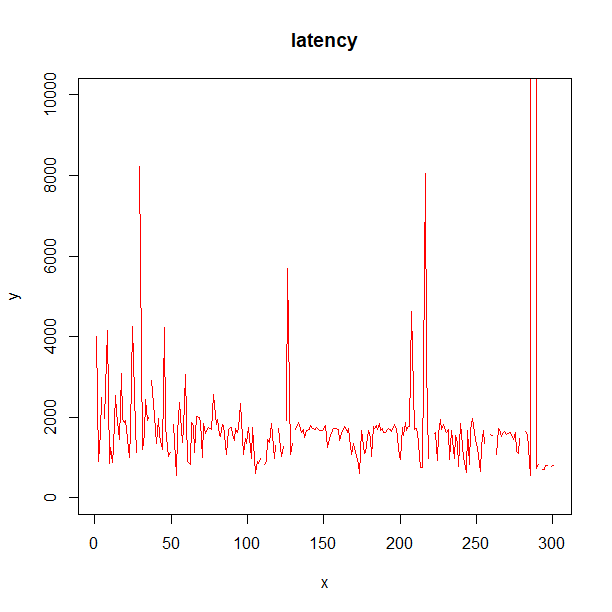
\includegraphics[width=0.5\textwidth]{images/ratelimit1.png}
  \caption{Senderate 1/sec, Testsystem A}
  \label{img:senderate1-A}
\end{figure}
Als naechstes wurde die Latenz zu einem entfernten RMQ Broker gemessen. Das System auf dem der entfernte Broker laeuft hat die selben spezifikationen wie das in \autoref{sec:testmachine} beschriebene. Die ausgemssenene Netzwerklatenz betrug 1ms. Die Senderate und Nachrichtengroesse sind wie oben beschrieben. Die Ergebnisse sind in \autoref{img:senderate1-B} zu sehen. Auch hier waechst die Latenz mit Ansteigen der Groesse. Im Unterschied zu ersten Messung ist die Latenz einer Nachricht groesser. 
%E
Die laengere Latenz in der zweiten Messung laesst sich auf die Netzwerklatenz zurueckfuehren. Somit ist neben der Nachrichtengroesse auch die Netzwerklatenz ein Faktor, der die Latenz einer Nachricht beeinflusst.

\begin{figure}
\center
  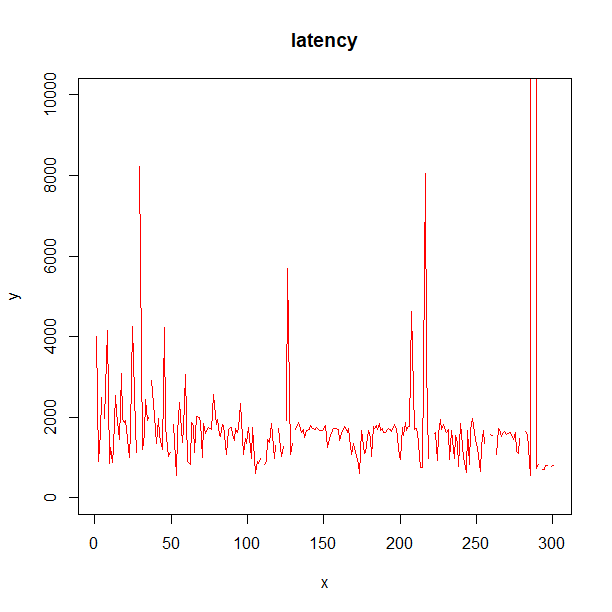
\includegraphics[width=0.5\textwidth]{images/ratelimit1.png}
  \caption{Senderate 1/sec, Testsystem A}
  \label{img:senderate1-B}
\end{figure}

\subsubsection{Nachrichtengroesse}
Im Folgenden sollen weitere Effekte im zusammenhang mit der Nachrichtengroesse untersuch werden. Dazu wurde die Limitierung der Senderate aufgehoben. Die Nachrichtengroessen variieren zwischen 100 Byte bis 1.000.000 Bytes.
%B
In \autoref{img:msgsize} sind die Auswirkung der Nachrichtengroesse auf die Senderate und die insgesamt gesendete Datenmenge zu sehen. dabei ist zu sehen, dass mit zunehmender groesse die Nachrichtenmenge die pro Sekunde gesendet werden kann, abnimmt. Gleichzeitig nimmt aber die insgesammt gesendete Datenmenge, in Bytes, zu. 
\begin{figure}
\center
  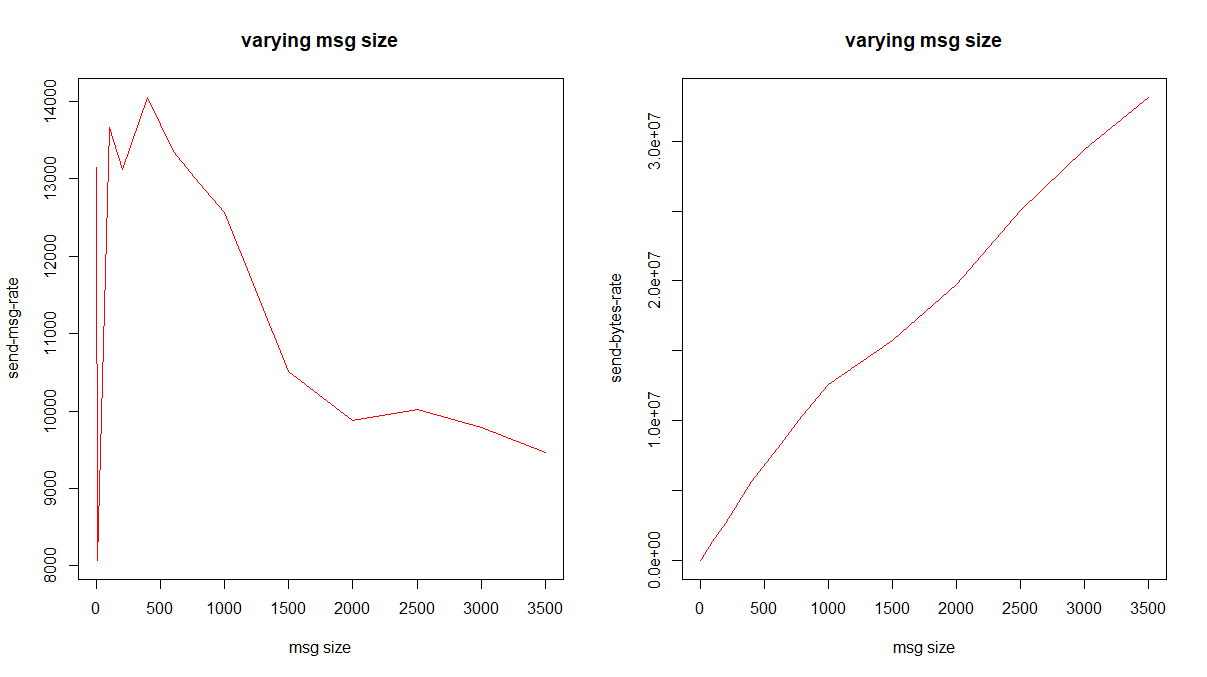
\includegraphics[width=1\textwidth]{images/msg-size.png}
  \caption{Senderate 1/sec, Testsystem B}
  \label{img:msgsize}
\end{figure}
%E
Dieser Effekt laesst sich darauf zurueckfuehren, dass bei groesseren Nachrichten der Broker weniger routing overhead hat.
%https://www.rabbitmq.com/blog/2012/04/25/rabbitmq-performance-measurements-part-2/

\subsubsection{Maximale zu sendende Datenmenge}
\label{sec:maxthroughput}
Nachdem die Effekte der zueahmende Nachrichtengroesse grprueft wurden, soll nun geprueft werden wie gross die insgesammt moegliche Datenmenge die gesendet und empfangen werden kann ist. Dazu wurden Nachrichten unterschiedlicher Groesse gesendet. Die Nachrichten waren zwischen 100 Bytes und 200000 Bytes (2MB) gross. Es wurden zwei Messungen durchgefuehrt. Die erste war mit einem Sender und keinem Empfaenger. Die zweite mit einem Sender und einem Empfaenger. 
%B
Die Ergebnisse sind in \autoref{img:maxByteThroughputA} zu sehen. Die Abbildung zeigt, dass wenn kein Empfaenger vorhanden ist, mit zunehmender Nachrichtengroesse die insgesamt gesendete Datenmenge an einen Wert bei ca. 230 MByte/s annaehert. Wenn ein Empfaenger vorhanden ist, naehert sich die Datenmenge an 174 MByte/s an.
\begin{figure}
\center
  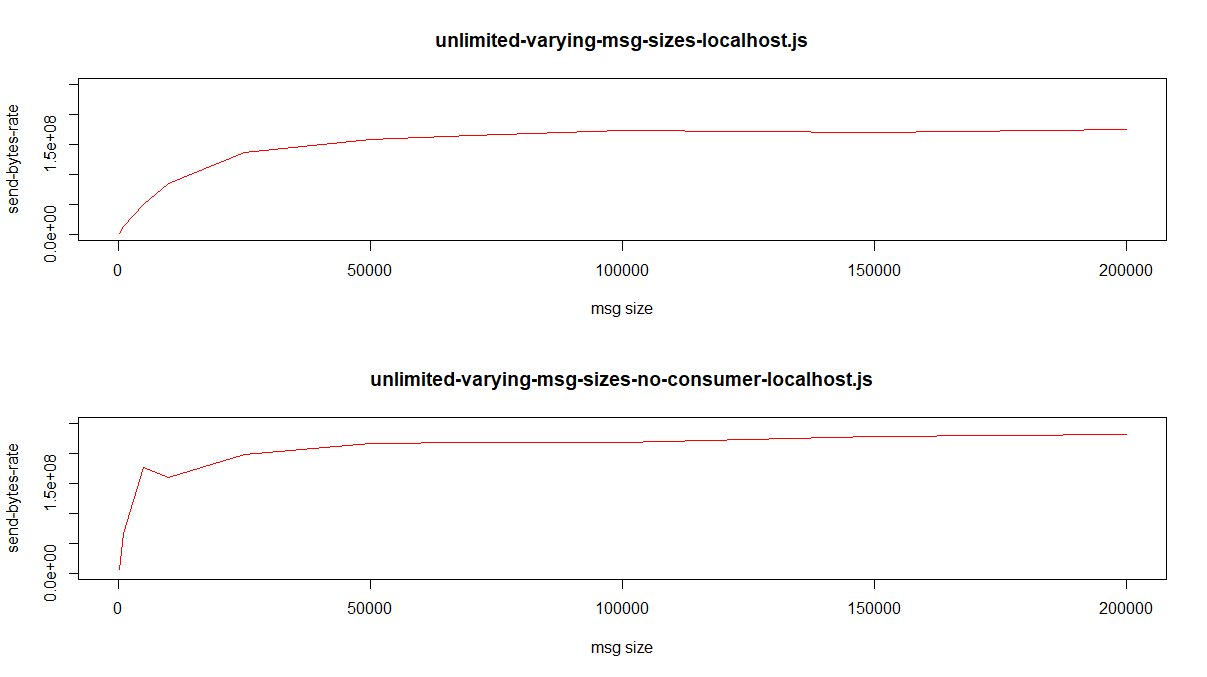
\includegraphics[width=1\textwidth]{images/max-byte-throughput-A.png}
  \caption{Max Datenmenge ca. 230/174 (kein Empfaenger/mit Empfaenger), Testsystem A}
  \label{img:maxByteThroughputA}
\end{figure}

Ein weiterer Effekt ist in \autoref{img:unlimitedLatency} zu sehen. Dabei ist zu sehen, dass die Latenz sinkt wenn mehr Nachrichten auf einmal gesendet werden.
\begin{figure}
\center
  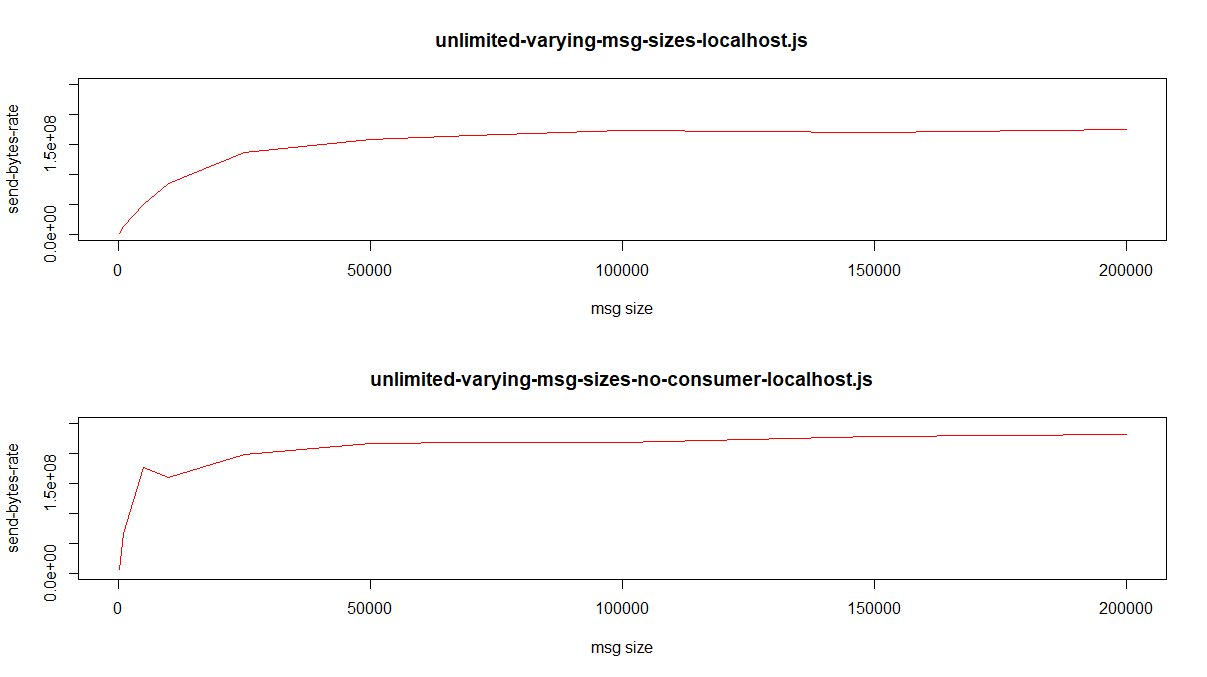
\includegraphics[width=1\textwidth]{images/max-byte-throughput-A.png}
  \caption{Max Datenmenge, Latenz, Testsystem A}
  \label{img:unlimitedLatency}
\end{figure}
Dieser Effekt laesst sich darauf zurueckfuehren, dass wenn mehrere Nachrichten auf einmal gesendet werden der Broker weniger routing overhead hat.

Die selbe Messung wurde an dem enfernten Testsystem B ausgefuehrt. %Auf Testsystem B wurde die selbe Messung durchgefuehrt. 
%Die Ergebnisse sind in \autoref{img:maxByteThroughputB} zu sehen. Die Datenmengen sind hier weniger gross. Bei dem Fall, dass kein Empfaenger vorhanden ist, naehert sich die  insgesamt gesendete Datenmenge an den Wert 1.1 MByte/s an. Wenn ein Empfaenger vorhanden ist, naehert sich die Datenmenge ebenfalls an 1.1 MByte/s an.
%\begin{figure}
%\center
 % 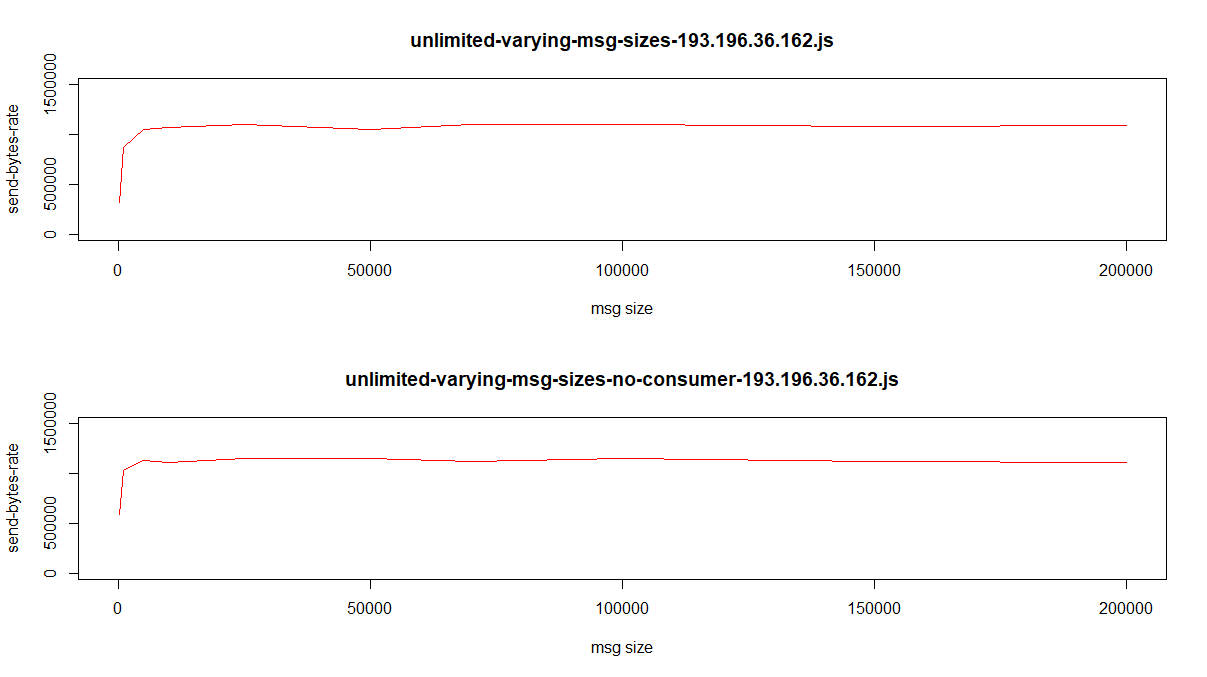
\includegraphics[width=1\textwidth]{images/max-byte-throughput-B.png}
%  \caption{Max Datenmenge ca. 1.1/1.1 (kein Empfaenger/mit Empfaenger), Testsystem B}
%  \label{img:maxByteThroughputB}
%\end{figure}
%E
%Die Messung zeigt einen limitierenden Faktor bzgl. der moeglich zu sendenden Nachrichtenmege. Dieser wird vor allem bei Testsystem B bemerkbar. Dort ist die moegliche zu sendende Datenmenge 1.1 Mbyte, was mit einer Upload Messung uebereinstimmt. Somit koennen in bestimmten Situationen nicht genug Daten gesendet werden und der Durchsatz wird limitiert.


%E
%Diese Unterschiede lassen sich auf die Netzwerklatenz zuruckfuehren. Im Testsystem A befinden sich Sender, Empfaenger und Brooker auf einer Maschine. Deshalb gibt es keine Netzwerklatenz und die Durchnittslatenz ist dementspraechend niedrig. Bei Testsystem B befinden sich der Brooker und der Empfaenger auf einer anderen Maschine. Deshalb spielt die Netzwerklatenz hier eine Rolle und die Latenz einzelner Nachrichten ist dementsprechend hoeher. Somit konnte ein Einflussfaktor fuer die Performanz identifiziert werden. 




\subsubsection{MaxLength}
\label{subsub:maxlength}
RMQ erlaubt es die Warteschlangen groesse zu limitieren. Ausserdem kann eine Strategie festgelegt werden, was mit ankommenden Nachrichten passieren soll. Im Standardfall wird der Kopf der Warteschlange verworfen. Dies sollte mit der folgenden Messung untersucht werden. Dazu wurde mehrere Warteschlange angelegt. Diese hatten eine Maximallaenge von 100, 5000 und 50.000. Die Groesse von 50.000 ist die RMQ standard groesse fuer Warteschlangen. Damit man die Auswirkung auf volle Warteschlangen sehen kann wurde die Sende- und Empfangsrate entsprechend angepasst. Die Senderate wurde auf 1000 und die Empfangsrate auf 100 Nachrichten die Sekunde eingestellt. Die Nachrichten groesse betraegt 100 Bytes.
%B
Die Ergebnisse sind in \autoref{img:maxlength} zu sehen. Zu sehen ist, dass die Latenz bei den begrenzten Warteschlangen ab einem bestimmte Zeitpunkt nicht weiter anwaechst. Die Latenz der unbegrenzten Warteschlange waechst dagegen immer weiter.
\begin{figure}
\center
  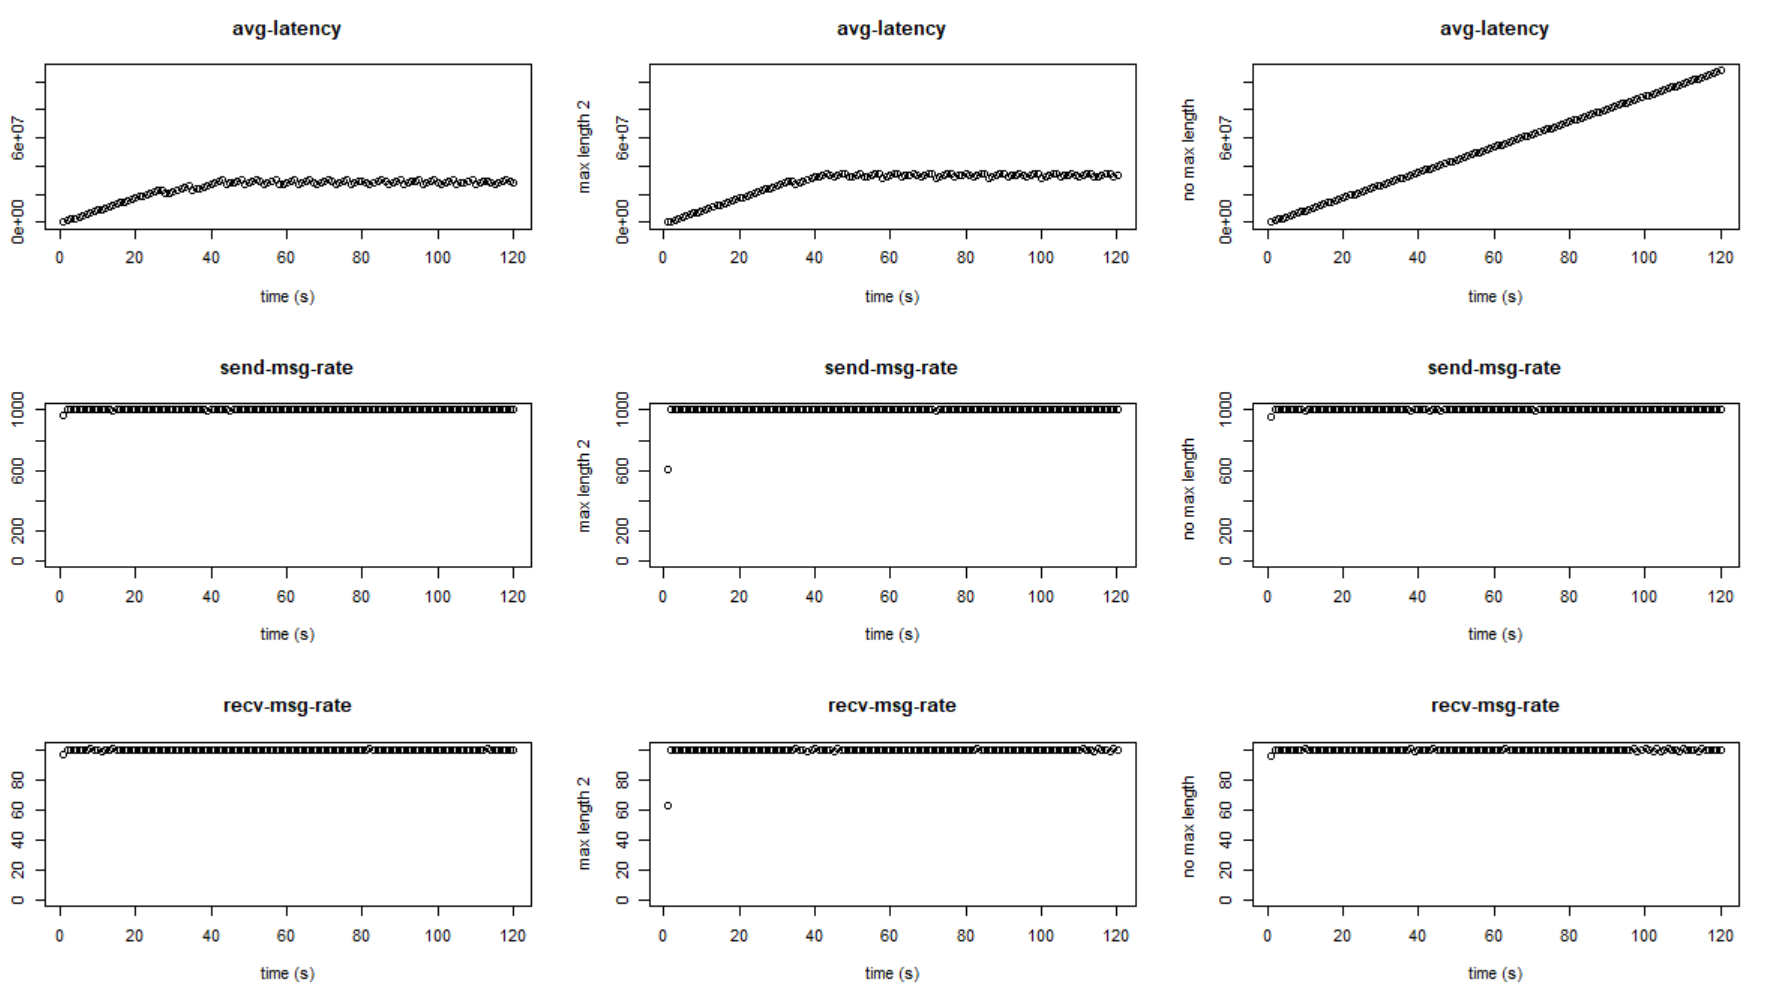
\includegraphics[width=1\textwidth]{images/max-length.png}
  \caption{Senderate 1000/sec, Empfangsrate 100/sec, Warteschlangenlaenge (links nach rechts) 100/5000/50.000}
  \label{img:maxlength}
\end{figure}
%E
Diese Konfiguration zeigt, dass die Warteschlangenbegrenzung einen Einfluss auf die Latenz hat und man diese gering halten kann, wenn man die Warteschlangengroesse begrenzt. Der Nachteil dabei ist, dass Nachrichten verworfen werden, sobald die Warteschlange voll ist. Somit hat auch die Warteschlangengroesse einen Einfluss auf die Performanz. 

%wenn Queue voll, dann wird Msgrate angepasst

%Flow alarm ab RabbitMQ 2.8.0+ bei Versionen davor verhlaehlt sich RMQ wie in (sec: Speicher ausgeschoepft)

\subsubsection{Speicher von RMQ ausgeschoepft}
Nachdem in der Messung davor die Laenge der Warteschlange betrachtet wurde, soll nun untersucht werden ob der Verfuegbare Speicher des Broker einfluss auf die Performanz hat. Dazu wurde auf der Testmaschine B die Hauptspeicher fuer RMQ auf 10 MB gesetzt.  
Sollte der verfuegbare Speicher des Broker ausgeschoepft sein, wird der MemoryAlarm aktiviert und der Broker blockiert ankommende Nachrichten, bis der Speicher wieder frei ist. Dies ist in (abb) zu sehen.
TODO beobachtung und Ergebnis

\subsubsection{Ansteigen der Queuelaenge}
TODO: \\
Sender 2 Nachrichten \\
Empfaenger 1 Nachricht \\
evtl. mehrere Verhaeltnisse \\
Fuellstand der Queue steigt an \\

\subsubsection{Lazy Queues}
%https://www.rabbitmq.com/lazy-queues.html
Seit RabbitMQ 3.6.0 erlaubt RMQ, dass Nachrichten einer Warteschlange direkt auf die Festplatte, anstatt in den Hauptspeicher, geschrieben werden. Diese Art von Warteschlange wird als Lazy-Queue bezeichnet. Das Ziel dabei ist, sehr lange Warteschlange zu unterstuetzen. Dies kann aus verschiedenen Gruenden noetig sein. 
\begin{itemize}
    \item Empfaenger koennen aus verschiedenen Gruenden ausfallen
    \item Ploetzlicher anstieg ankommender Nachrichten
    \item Empfaenger sind langsamer als normal
\end{itemize}
Das heisst die Hauptziele bei dieser Konfiguration sind vorallem Zuverlaessigkeit. In der naechsten Messung soll untersucht werden ob diese Konfiguration Auswirkungen auf die Performanz hat. Die Senderate wurde auf eine Nachricht pro Sekunde limitiert. Die groesse der gesendeten Nachrichten varriieren zwischen 100 Byte und 100.000 Bytes.
%B
In \autoref{img:lazy} sind die Ergebnisse der Messung zu sehen. Ausserdem sind in der Abbildung die Ergebniss aus der Messung aus \autoref{sec:rate1} eingetragen. Zu sehen ist, dass die Latenz mit Lazy Warteschlangen groesser ist, als ohne.
\begin{figure}
\center
  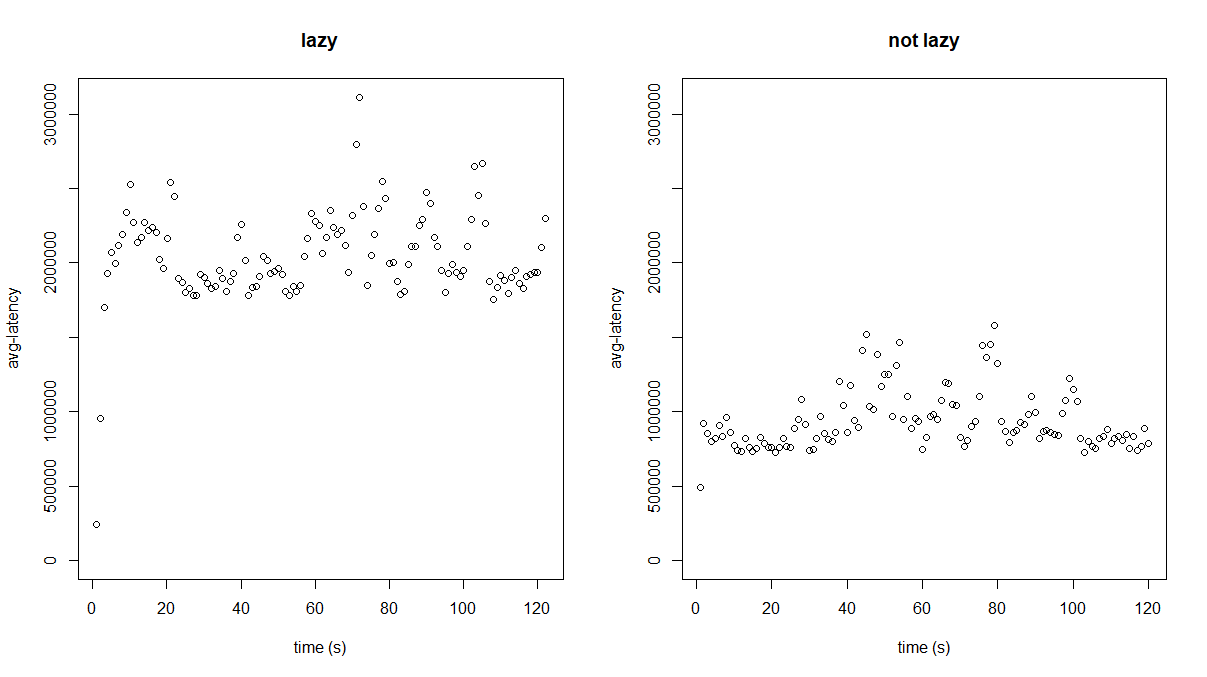
\includegraphics[width=1\textwidth]{images/lazy.png}
  \caption{Lazy Queue vs not Lazy Queue}
  \label{img:lazy}
\end{figure}
%E
Grund hierfuer ist das die Nachrichten auf die Festplatte anstatt in den Hauptspeicher geschrieben werden. Somit hat der Ort an den Nachrichten gespeichert werden einen Einfluss auf die Performanz.



\subsubsection{Mehrere Empfaenger}
In \autoref{subsub:maxlength} war bereits zu sehen, dass volle Warteschlangen einen Einfluss auf die Latenz haben. In dieser Messung soll geprueft werden ob mehrere Empfaenger eine Warteschlange genauso schnell abarbeiten koennnen wie ein einzelner und somit die Latenz gemeinsam in den Griff bekommen koennen. Dazu wurde die Senderate eines Senders auf 1000 Nachrichten und die Empfangsrate auf 200 Nachrichten pro Sekunde limitiert. Alle Empfaenger greifen auf die selbe Warteschlange zu. Ausserdem wurde eine Referenzmessung mit einem Sender und einem Empfaenger mit einer Empfangsrate von 1000 durchgefuehrt.
%B
In \autoref{img:varyingConsumer} sind die Ergebnisse der Messung zu sehen. Darin ist zu sehen, dass ein Empfanger mit gedrosselter Empfangsrate nicht hinterherkommt die Warteschlange abzuarbeiten und somit die Latenz sehr schnell steigt. Bei zwei Empfaenger, mit einer gemeinsamen Empfangsrate von 400 Nachrichten die Sekunde, steigt die Latenz nicht ganz so schnell, aber auch hier kommen die Empfanger nicht hinterher die Warteschlange abzuarbeiten. Mit fuenf Empfaenger und einer gemeinsamen Empfangsraten von 1000 Nachrichten, schaffen sie es die Warteschlange abzuarbeiten. Im Vergleich zu der Referenzmessung mit einem Empfaenger, beinhaltet die Messung mit mehreren Empfaengern einige Schwankungen.
\begin{figure}
\center
  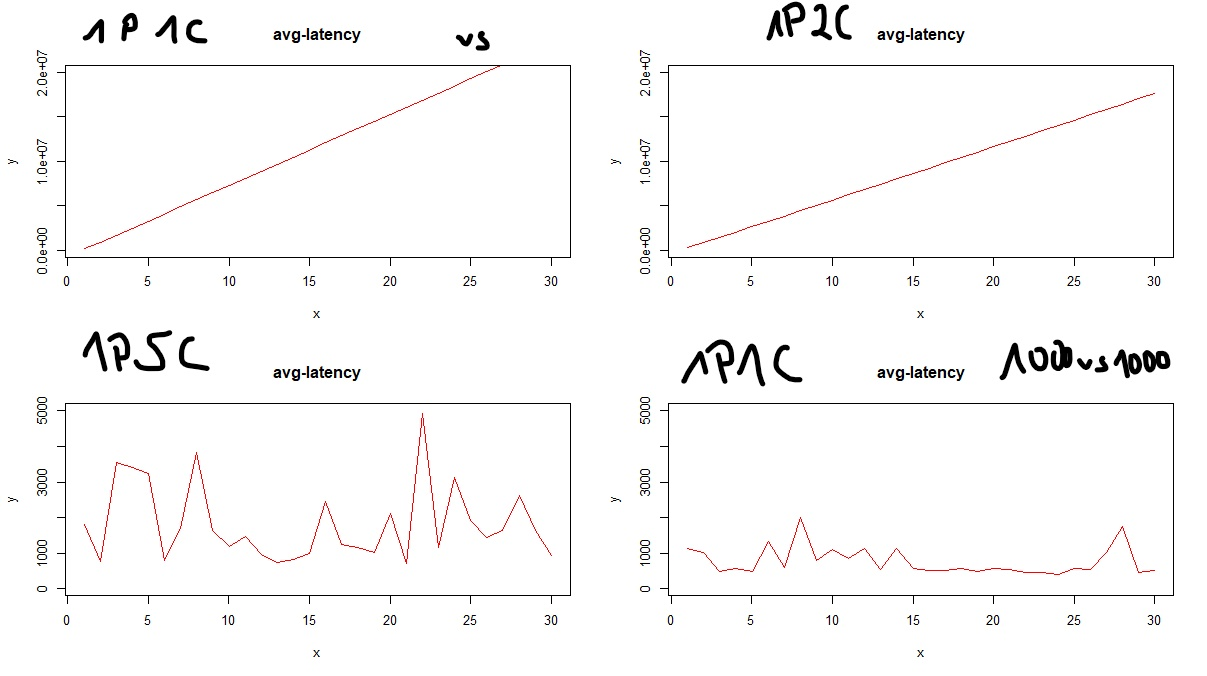
\includegraphics[width=1\textwidth]{images/varyingConsumer.jpg}
  \caption{Verschiedene Empfaenger Anzahl}
  \label{img:varyingConsumer}
\end{figure}
%E
Diese Messung zeigt, dass mehrer Empfaenger eine Warteschlange genauso schnell abarbeiten koennen wie ein einzelner. Die Schwankungen lassen sich mit der synchronisation der Empfaenger erklaeren. Da diese Schwankungen minimal sind, kann dieser Effekt vernachlaessigt werden.

\subsubsection{Mehrere Sender}
Diese Messung soll ueberpruefen ob es einen Unterschied macht ob mehrere Sender die gleiche Performanz schaffen, wie ein einzelner. Dazu wurde als Referenz ein Sender mit einer Senderate von 5000 Nachrichten die Sekunde und 5 Sender mit jeweils 1000 Nachrichten die Sekunde untersucht. 
%B
In \autoref{img:varyingProducer} sind die Ergebnisse dieser Messung zu sehen. 
\begin{figure}
\center
  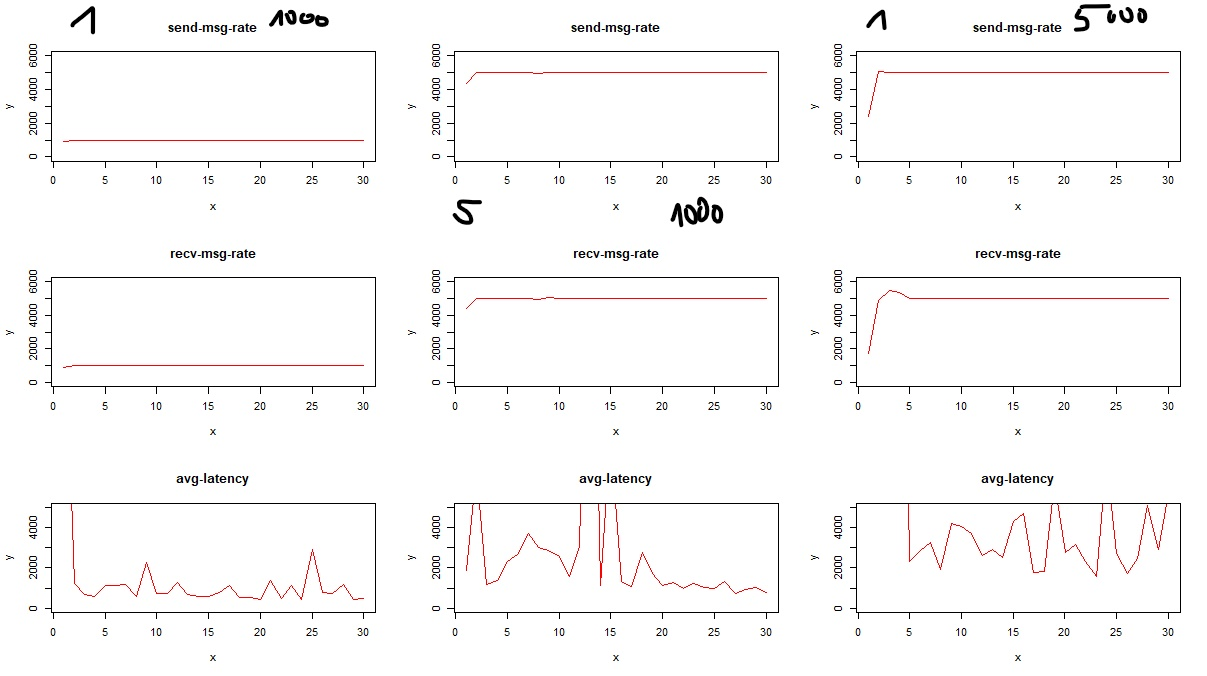
\includegraphics[width=1\textwidth]{images/varyingProducer.jpg}
  \caption{Verschiedene Sender Anzahl}
  \label{img:varyingProducer}
\end{figure}
%E
Diese Messung zeigt, dass er vernachlaessigbar ist ob ein Sender oder mehrere Sender benutzt werden um eine bestimmte Senderate zu erreichen. 
%A
%In einer weiteren Messung sollte Ausserdem geprueft werden, ob mehrere Sender ohne Sendelimit mehr Nachrichten senden koennen als ein Sender. Dazu wurde der selbe Versuchsaufbau wie oben gewaehlt mit dem Unterschied, dass diesmal die Senderate nicht eingeschraenk wurde.
%B
%In \autoref{img:varyingProducerMaxThroughput} sind die Ergebnisse dargestellt. Dabei ist zu sehen, dass die 5 Sender zusammen genauso viele Nachrichten senden wie ein Sender allein. Ausserdem ist die Latenz im Fall der 5 Sender um ein 5faches groesser als bei einem Sender.
%\begin{figure}
%\center
%  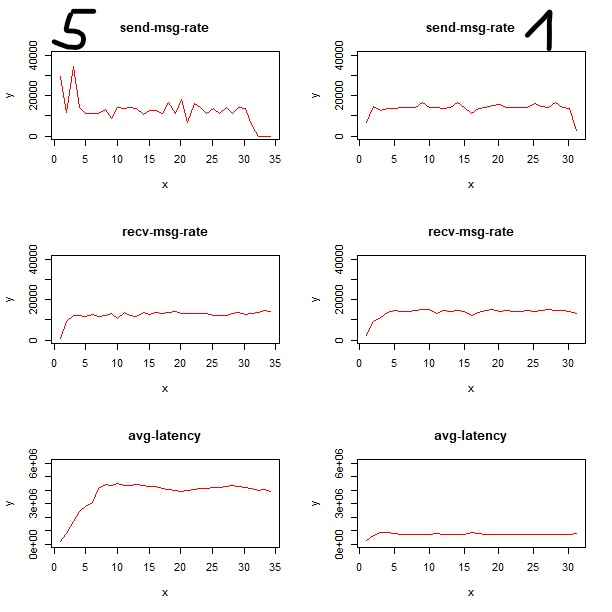
\includegraphics[width=1\textwidth]{images/varyingProducerMaxThroughput.jpg}
%  \caption{Verschiedene Sender Anzahl}
%  \label{img:varyingProducerMaxThroughput}
%\end{figure}
%E
%Das die 5 Sender jeweils nur 1/5 der moeglichen Senderate senden, kann dadurch erklaert werden, dass das Testsystem nicht mehr als eine bestimmte Rate an Nachrichten senden kann. D.h. das es keinen Unterschied macht ob ein Sender oder mehrere Sender Nachrichten senden. DIeses Verhalten kann sich aendern, wenn sich verschiedene Sender auf verschiedenen Maschinen befinden. (evtl noch Messung durchfuehren um zu zeigen) 


%Ableitung von ResourceDemands -> Regressionsfkt

%\subsection{ActiveMQ}
%ActiveMQ \cite{activeMQ} ist eine Open-Source-MOM, die seit 2004 kontinuierlich weiter entwickelt wird. ActiveMQ ist in Java geschrieben und implementiert den Java Message Service (JMS) \cite{jms}. Dabei handelt es sich um eine Programmierschnittstelle zur Ansteuerung einer MOM. Dabei soll eine lose gekoppelte, verlässliche und asynchrone Kommunikation zwischen den Komponenten einer verteilten Anwendung ermöglicht werden. ActiveMQ verfügt außerdem über mehrere Betriebsarten für hohe Verfügbarkeit und einen robusten horizontalen Skalierungsmechanismus. Darüber hinaus ist es sehr flexibel in der Konfiguration und unterstützt eine Vielzahl von Transportprotokollen, darunter auch AMQP.

\subsection{Zusammenfassung}
welche Einflussfaktoren konnnten identifiziert werden und werden weiter betrachtet? \\
Nachrichtengroesse hat einfluss auf Latenz, Senderate und gesendete Datenmenge \\
%Througput der Verbindung (linking Ressource)\\
%Msg rate des Senders und Empfaengers (ankunftsrate im Usage modell) \\
%Nachrichtengroesse und ihre Latenz (response time einer Nachricht) \\
Netzwerklatenz \\
Moegliche Datenmenge ist durch Netzwerk begrenzt\\
Ob Nachrichten in HS oder HDD gespeichert werden (lazy queues) \\
Kein Unterschied ob ein oder mehrere Sender/Empfaenger Warteschlange fuellen/abarbeiten \\

welche weiteren Einflussfaktoren gibt es, die aus bestimmten gruenden nicht betrachtet werden (koennen)\\
wenn system mehr Nachrichten auf einmal sendet/empfaengt sinkt latenz wieder \\
RMQ hat auch Prefetch von Nachrichten. Wird nicht betrachtet (zeit und trotzdem nicht so gut wie kafka) \\
Latenz steigt an, wenn die queue gefuellt wird \\
- benoetigt tracken einer Nachricht durch das system \\
- explizite Queue Modellierung, mit groesse und fuellstand \\

\subsection{Kafka}
Beschreibe Benchmark
\subsubsection{Latenz einer Nachricht}
1 Msg, fetch 1 => 317 ms \\
(paar zwischen schritte)
10000000 Msg fetch 1 => 4 mikrosek pro msg\\

Grund: seek time
\subsubsection{Latenz mehrere Nachrichten}
4 mikrosek bis 1.14 mikrosek als grenze \\

%\subsubsection{Mehrere Empfaenger}
%\subsubsection{Mehrere Sender}
\subsection{Zusammenfassung}
welche Einflussfaktoren konnnten identifiziert werden und werden weiter betrachtet? \\
fetch size \\
welche weiteren Einflussfaktoren gibt es, die aus bestimmten gruenden nicht betrachtet werden \\
\section{Vergleich von MOMs}
Kafka eignet sich nicht fuer einzelne Nachrichten \\
- deutlich langsamer als RMQ \\
- pull vs push \\
- Kafka deutlich schneller, sobald mehr Nachrichten verschickt werden \\
- Speicher Begrenzt durch HDD und nicht HS \\

%--	Vergleich: https://stackshare.io/stackups/activemq-vs-kafka-vs-rabbitmq  \\


